\section{Thermal mass estimation}
\label{ch:thermtool}
Decelerating an entry vehicle requires a thermal protection system. This system will contribute to a large extend to the mass of the entire vehicle. Therefore, a thermal protection system (\gls{tps}) has a critical impact on the mission an should be selected properly. This section will analyse the \gls{tps} of the five trade-off concepts with the use of a thermal protection tool. First the tool will be described in more detail. Afterwards it is described how the tool is verified and validated. In the third section, this tool will be used to analyse different lay-ups for the concepts under anlysis. As a result,the \gls{tps} masses for differnt concepts can be determined. Lastly, concluions and recomendations.

\subsection{Method of thermal analysis}
A mass estimations of the \gls{tps} requires analysis due to heat transfer in the heat shield. Enable to analyse different lay-ups in a short amount of time, it will be usefull to make use of a \gls{tps} tool. The working principles of this tool are describes in detail in this section.

\subsubsection{Assumptions}


\subsubsection{Leading equations}
The problem is modeled as a one-dimensional multilayer layup which can provide the accuracy needed or this stage of concept analysis as described in the assumptions. A description of the implementation of this model is given by Smith {Smith2011}. The model is illustrated in Figure \ref{fig:1dthermal}. The figure shows the different methods of heat transfer in the model. There is heat radiating away from the surface, convective heating or heat flux from the aerodynamic effects and heat conduction within the layers.

\begin{figure}[H]
	\centering
	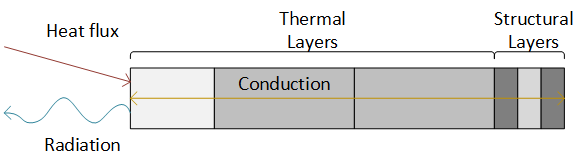
\includegraphics[width = 1.0\textwidth]{Figure/1dthermal.png}
	\caption{1D thermal model}
	\label{fig:1dthermal}
\end{figure}
\subsubsection{Input}
Lucas
\subsubsection{Output}
Suthes


\subsection{Verification \& Validation}

\subsubsection{Verification}
Suthes
\subsubsection{Validation}



\subsection{Results per concept}



\subsection{Conclusion \& recomendations}
